%!TEX root=./report.tex
\newpage
\section{Appendix}
\begin{figure}[h!]
	\centering
	\includegraphics[width=0.49\linewidth]{cifar10}
	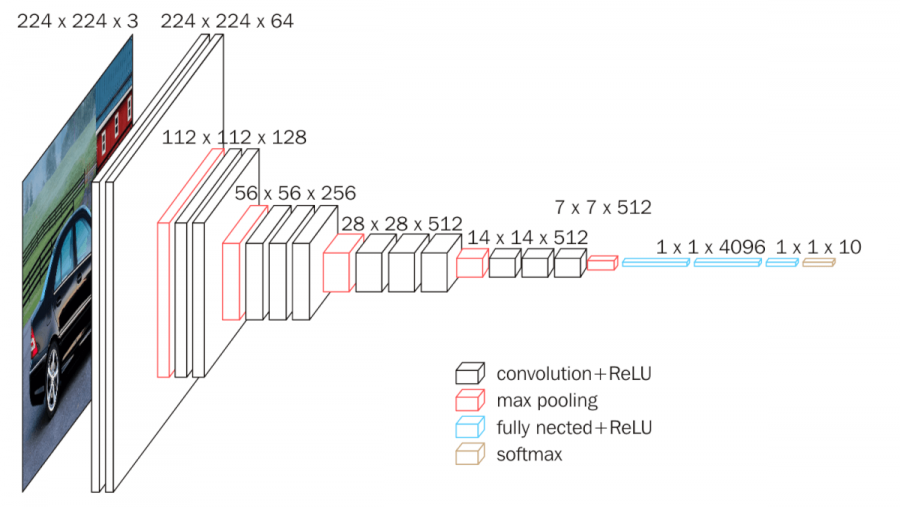
\includegraphics[width=0.49\linewidth]{vgg16}
	\caption{Left: A subset of the CIFAR-10 small image data set with ten classes. Right: The used implementation of the VGG-16 network with batch normalization. \cite{cifar10, vgg16}}	
	\label{fig:cifar-vgg}
\end{figure}

\begin{figure}[h!]
	\centering
	\includegraphics[width=0.45\linewidth]{mnist}
	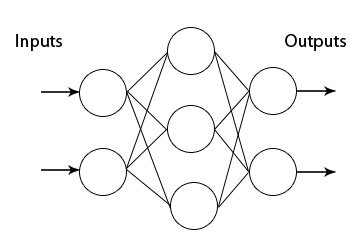
\includegraphics[width=0.45\linewidth]{two_layer_perceptron}
	\caption{Left: A subset of the MNIST handwritten digit data set. Right: An exemplary two layer perceptron with one input layer, one hidden layer of hidden unit size three and one output layer. \cite{mnist, two-layer-perceptron}}	
	\label{fig:mnist-two-layer}
\end{figure}

\begin{figure}[h!]
	\centering
	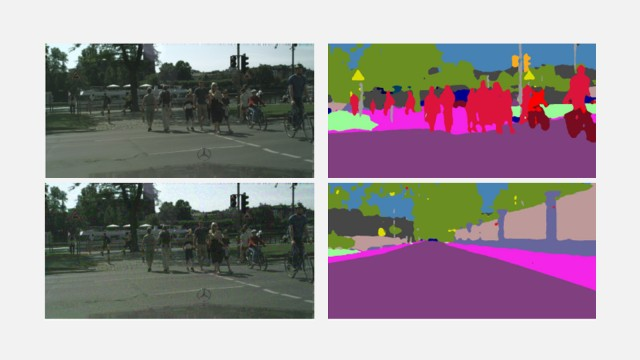
\includegraphics[width=0.8\linewidth]{bosch}
	\caption{Upper row: The original image (left) and the correct segmentation mask (right). Lower~row: The image with some additive adversarial perturbation barely visible to the human eye (left) and the corresponding wrong segmentation mask (right). \cite{metzen2017universal}}	
	\label{fig:adversarial-perturbations}
\end{figure}